\documentclass{article}
\usepackage{scribe}
\usepackage{epsfig}
\usepackage{amsmath}
\renewcommand{\Pr}[1]{\textrm{\textup{Pr}}\left( #1 \right)}
\newenvironment{slist}
  {\begin{list}{$\bullet$}{\parsep0pt\itemsep0pt\topsep0pt}}
  {\end{list}}

\title{Linear Programming Algorithms\\ 6.854 Scribe Notes \#14}
\date{October 18, 2004}
\author{Lecturers: David Karger\\ Scribe: David Schultz}

\begin{document}

%%%%%%%%%%%%%%%%%%%%%%%%%%%%%%%%%%%%%%%%%%%%%%%%%%%%%%%%%%%%%%%%%%%%%%
% Your notes start here!
%%%%%%%%%%%%%%%%%%%%%%%%%%%%%%%%%%%%%%%%%%%%%%%%%%%%%%%%%%%%%%%%%%%%%%
%
% For theorems, lemmas, definitions, remarks, etc. use commands
% {\theorem{...}}, {\lemma{...}}, {\definition{...}}, etc.
% For proofs, use \begin{proof} ... \end{proof}
%
% For postscript figures (.ps) use the following block:
%
% \begin{figure}[h]
% \begin{center}
% \mbox{\psfig{figure=notes-nn-fig-mm.ps}}
% \caption{A very nice picture.}
% \label{fig:picture}
% \end{center}
% \end{figure}
%

% For encapsulated postscript figures (.eps) use the following block:
%  (also change documentstyle line )
% \begin{figure}[h]
% \begin{center}
% \mbox{\epsfbox{notes-nn-fig-mm.eps}}
% \caption{A very nice picture.}
% \label{fig:picture}
% \end{center}
% \end{figure}
%


%%%%%%%%%%%%%%%%%%%%%%%%%%%%%%%%%%%%%%%%%%%%%%%%%%%%%%%%%%%%%%%%%%%%%%


\section{Algorithms for Linear Programming}

\subsection{Last Time: The Ellipsoid Algorithm}

Last time, we touched on the ellipsoid method, which was the first
polynomial-time algorithm for linear programming.  A neat property of
the ellipsoid method is that you don't have to be able to write down
all of the constraints in a polynomial amount of space in order to use
it.  You only need one violated constraint in every iteration, so the
algorithm still works if you only have a \textit{separation oracle}
that gives you a separating hyperplane in a polynomial amount of time.
This makes the ellipsoid algorithm powerful for theoretical purposes,
but isn't so great in practice; when you work out the details of the
implementation, the running time winds up being $O(n^6\log nU)$.

\subsection{Interior Point Algorithms}

We will finish our discussion of algorithms for linear programming
with a class of polynomial-time algorithms known as \textit{interior
point algorithms}.  These have begun to be used in practice recently;
some of the available LP solvers now allow you to use them instead of
Simplex.

The idea behind interior point algorithms is to avoid turning corners,
since this was what led to combinatorial complexity in the Simplex
algorithm.  They do this by staying in the interior of the polytope,
rather than walking along its edges.  A given constrained linear
optimization problem is transformed into an unconstrained gradient
descent problem.  To avoid venturing outside of the polytope when
descending the gradient, these algorithms use a potential function
that is small at the optimal value and huge outside of the feasible
region.

\begin{figure}[h]
\begin{center}
  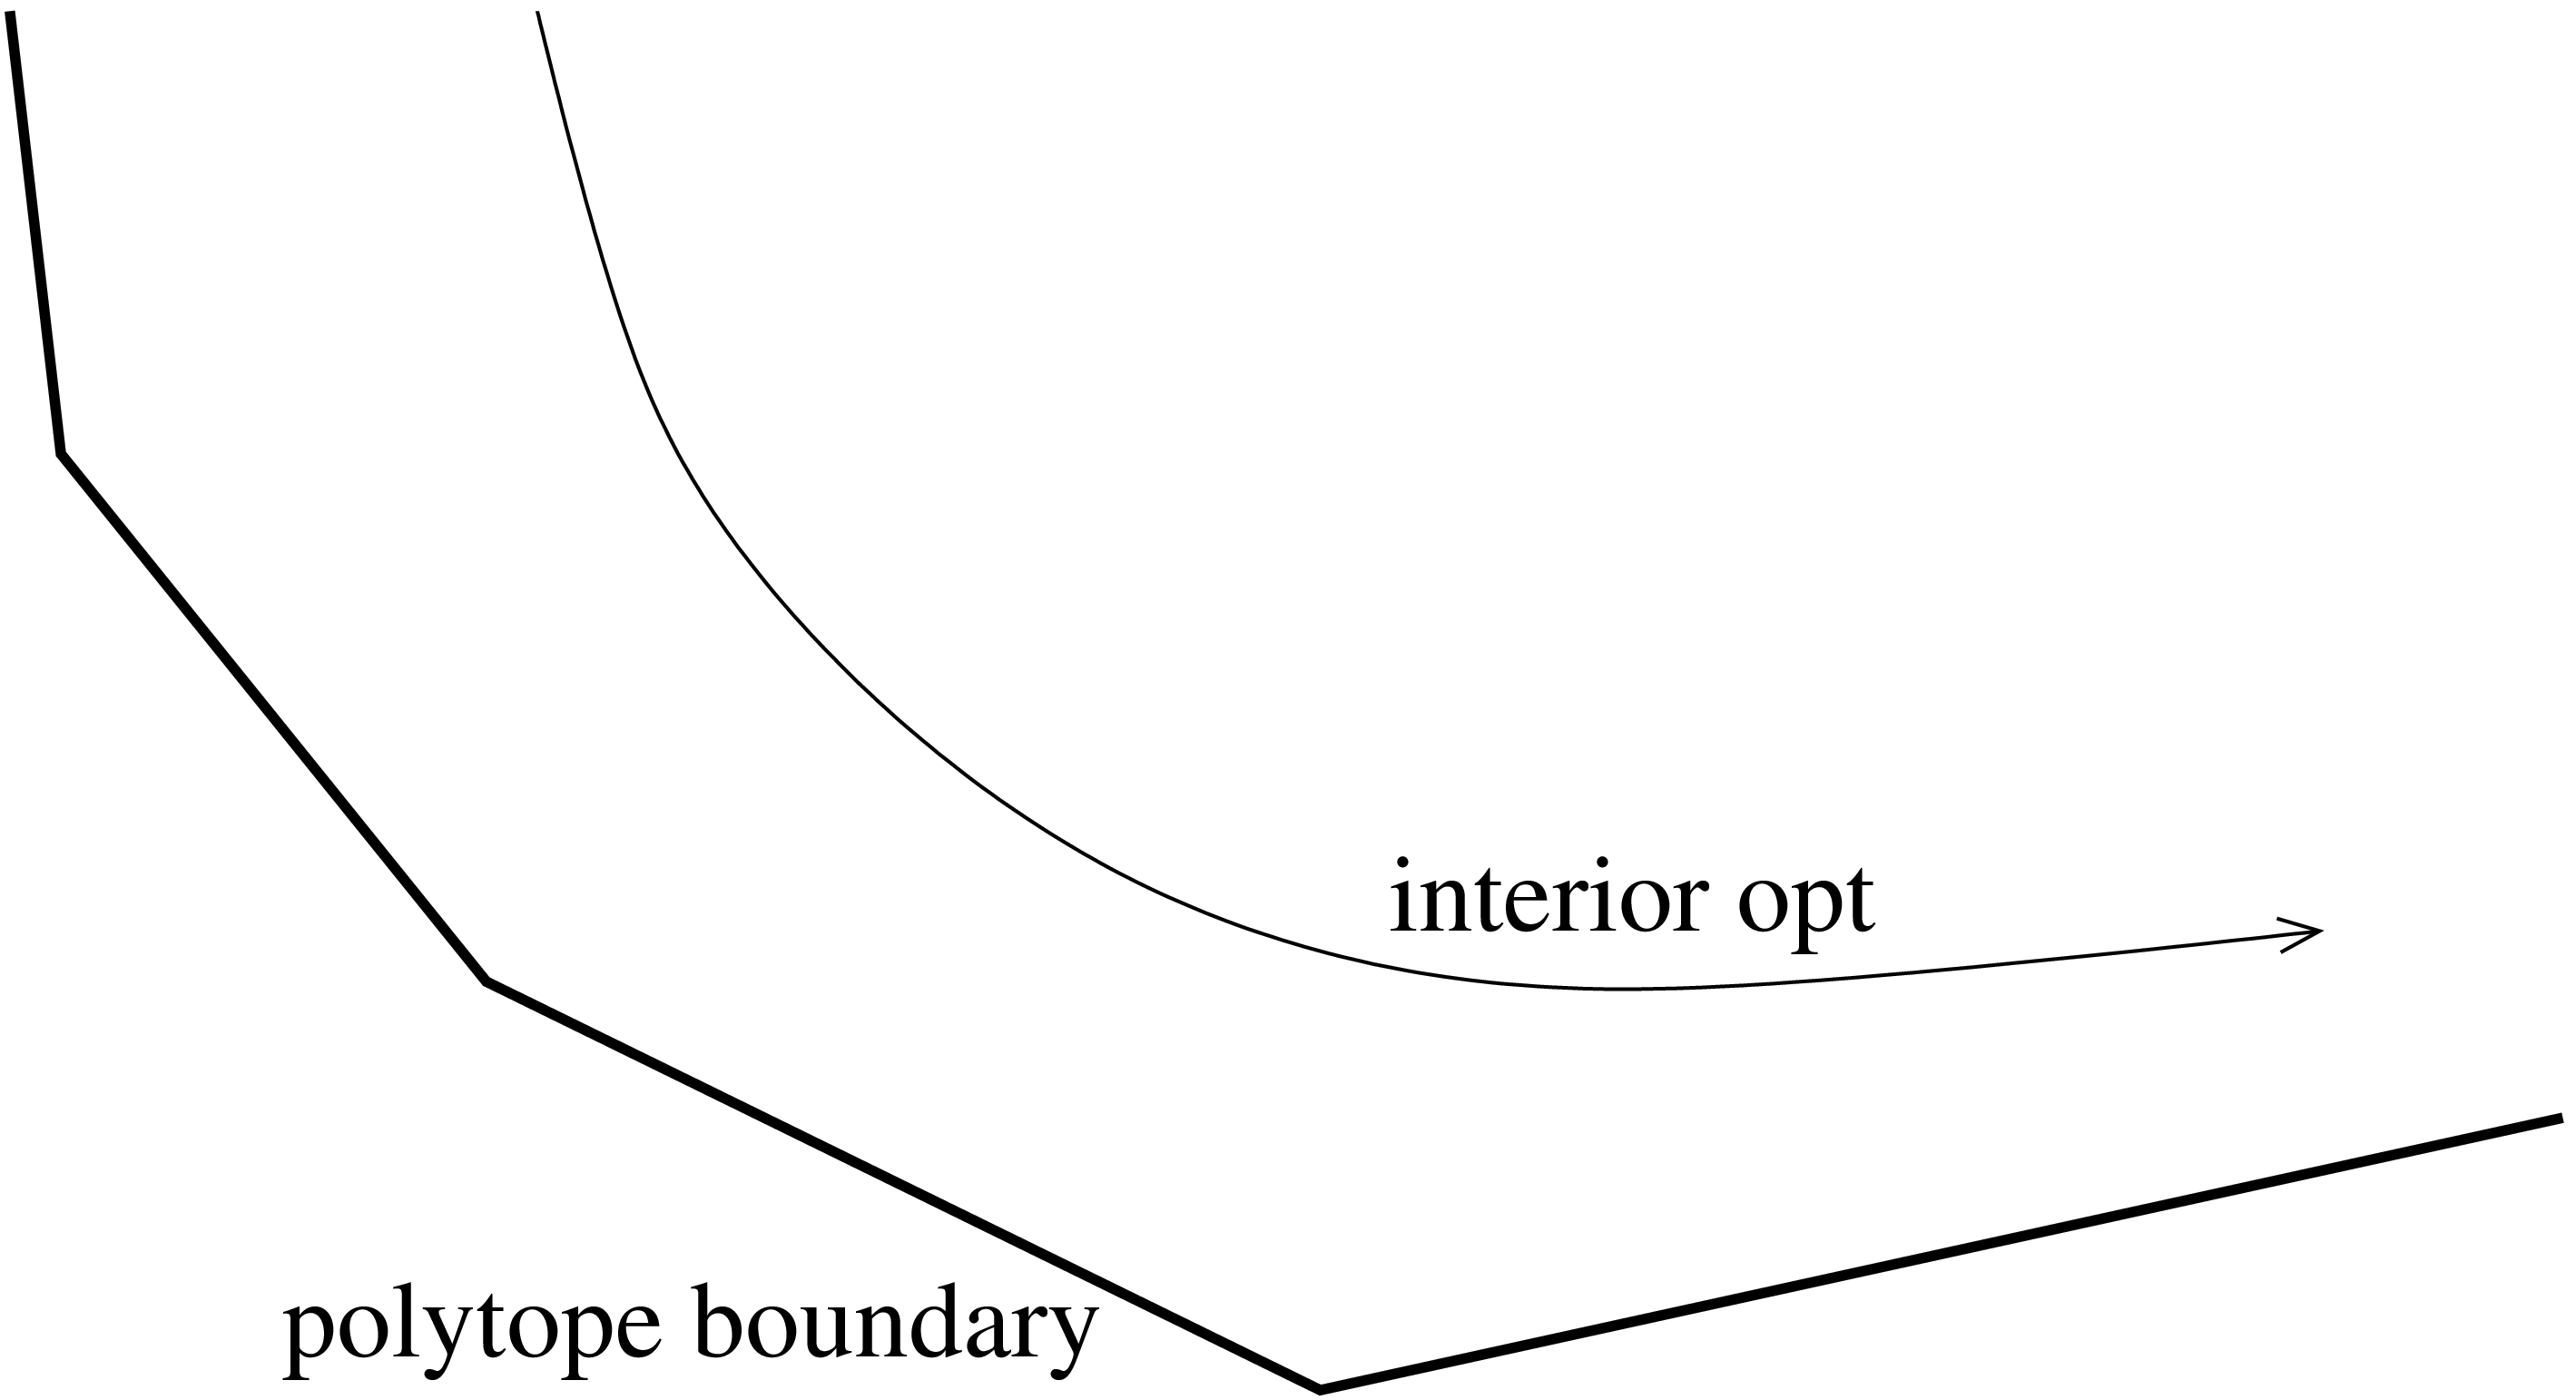
\includegraphics{lp-1.png}
  \caption{An interior point search.}
  \label{fig:interiorpt}
\end{center}
\end{figure}

To make this idea more concrete, let us consider a specific interior point
algorithm due to Ye.  Consider the following linear program:
{\setlength\arraycolsep{2pt}
\begin{eqnarray*}
\textrm{minimize\quad} & cx &\\
\textrm{subject to\quad} & Ax &=  b\\
                         & x &\ge 0\\
\end{eqnarray*}
}
The dual of this program can be written with slack variable $s$ as follows:
{\setlength\arraycolsep{2pt}
\begin{eqnarray*}
\textrm{maximize\quad} & yb &\\
\textrm{subject to\quad} & yA + s &=  c\\
                         & s &\ge 0\\
\end{eqnarray*}
}
Ye's algorithm solves the primal and the dual problem simultaneously;
it approaches optimality as the duality gap gets smaller.
The algorithm uses the following potential function:
\[
\phi = A\ln xs - \sum\ln x_i - \sum\ln s_i
\]
The intent of the $A\ln xs$ term is to make the optimal solution
appealing.  Note that $\ln xs$ approaches $-\infty$ as the duality gap
approaches 0.  The two subtracted terms are \textit{logarithmic
barrier functions}, so called because their purpose is to make
infeasible points unappealing.  When one of the $x_i$ or $s_i$ is
small, they add a large amount to the potential function.  When one of
the $x_i$ or $s_i$ is negative, these functions are infinitely
unappealing.  The constant $A$ needs to be made large enough that the
pull towards the optimal solution outweighs the tight constraints at
the optimal point.

To minimize $\phi$, we use a gradient descent.  We need to argue that
the number of gradient steps is bounded by a polynomial in the size of
the input.  It turns out that this can be done by arguing that in each
step, we get a large improvement.  Finally, when we reach a point that
is very close to the optimum, we use the trick from last time to move
to the closest vertex of the polyhedron.

\subsection{Conclusion to Linear Programming}

Linear programming is an incredibly powerful sledgehammer.  Just about
any combinatorial problem that can be solved can be solved with linear
programming (although many of these special cases of linear
programming can be solved more quickly by other methods).  For the
rest of the lecture, however, we will look at some of the problems
that cannot be solved by linear programming.

% [punya, 12/13/2006] The remainder of this material is commented out because
%                     it is covered in another set of lecture notes.

% \vfill\eject
% 
% \section{Polynomial-Time Approximation Algorithms}
% 
% $NP$-hard problems are a vast family of problems that (to the best of
% our knowledge) cannot be solved in polynomial time.  It is important
% to be able to identify such problems because it tells you where to
% direct your efforts.  In this class, we will not prove any of these
% problems to be $NP$-hard; you should take 6.840 to learn how to do that.
% \footnote{Briefly, $P$ is the set of problems solvable in
%   polynomial time, and $NP$ is a particular superset of $P$.  A
%   problem is $NP$-hard if it is at least as hard as all problems in
%   $NP$, and $NP$-complete if it is in $NP$ and it is also $NP$-hard.
%   An unproven but generally accepted conjecture, which we will assume
%   is true, is that $P\ne NP$.}
% 
% Instead, the question we concern ourselves with is how to cope once it
% has been proved that a problem is $NP$-hard.  Here are three possible
% strategies:
% 
% \begin{itemize}
% \item
% Assume that the input is random, and prove that an algorithm will
% perform well in the average case.  For example, the $NP$-hard problem
% of finding the maximum clique in a graph can be solved efficiently by
% this argument because the maximum clique in a randomly-chosen graph
% is small.  This argument is often used in practice, but it has the
% problem that not everyone will agree that the input distribution is
% random.
% 
% \item Run a super-polynomial algorithm anyway.  Techniques such as
% branch-and-bound (known as $A^*$ search in the AI world) allow you to
% enumerate options in a way that lets you skip most of the problem
% space.  However, the desired complexity bounds on these algorithms are
% usually not provable, and even ``slightly'' super-polynomial
% is often too much to be practical.
% 
% \item Settle for a suboptimal solution (an approximation) that can be
% found in polynomial time, and prove that this solution is ``good
% enough''.  This is the technique that we will look at in the rest of
% the lecture.
% \end{itemize}
% 
% \subsection{Preliminaries}
% 
% \begin{definition} An \textbf{optimization
%   problem} consists of:
%   \begin{description}
%   \item A set of instances $I$
%   \item A set of solutions $S(I)$
%   \item An objective function\footnote{The
% restriction that the range of the objective function is
% {\boldmath$R$} might be limiting in some situations, but most problems
% can be formulated this way.}
%  $f: S(I)\to \mbox{\boldmath
%   $R$}$
%   \end{description}
%   The problem is to find $s\in S(I)$ that maximizes (or minimizes)
%   $f(s)$.
% \end{definition}
% 
% Some technicalities: When we come to analyze the complexity of such
% problems, we will assume that all inputs and the range of $f$ are in
% the rational numbers.  We will also assume that if $\sigma$ is an
% optimal solution, then $f(\sigma)$ is polynomial in the number of bits
% in the input.  Our goal will be to find algorithms that take a
% polynomial amount of time in the representation of the input in bits.
% 
% \begin{example} \textbf{Graph Coloring} is an optimization problem
%   with the following form:
%   \begin{description}
%   \item $I$: graphs
%   \item $S(I)$: assignments of colors to each vertex such that
%                 no neighbors have the same color
%   \item $f(s)$: number of colors used in $s$
%   \end{description}
% \end{example}
% 
% Often when people talk about $NP$-hard problems, they are referring to
% decision problems, which are algorithms for which the output is
% \texttt{yes} or \texttt{no}.  For instance, a decision version of
% Graph Coloring is the problem of determining whether a graph is
% 3-colorable.  We need a notion of $NP$-hardness that applies to
% optimization problems as well.
% 
% \begin{definition} \textbf{{\boldmath{$NP$}}-hardness:} An optimization
%   problem is $NP$-hard if it can be used as a subroutine to solve an
%   $NP$-hard decision problem in polynomial time, with the optimization
%   problem used as a black box.
% \end{definition}
% 
% \begin{definition} An \textbf{approximation algorithm} is \textit{any}
%   algorithm that gives a feasible solution to an optimization problem.
% \end{definition}
% 
% The above definition sounds a bit silly.  For instance, a valid
% approximation algorithm for Graph Coloring is to color each vertex
% with its own color.  In order to formulate \textit{useful}
% approximation algorithms, we need a way to be able to differentiate
% them based on the ``goodness'' of the approxmiation.  In the rest of
% the lecture, we will consider two ways to measure ``goodness.''
% 
% \subsection{Absolute Approximations}
% 
% One way to compare approximation algorithms is to measure the
% solutions they find relative to the optimal solution, $OPT(I)$.
% 
% \begin{definition} $A$ is a \textbf{{\boldmath$k$}-absolute
%     approximation algorithm} if $|A(I) - OPT(I)| \le k$.
% \end{definition}
% 
% The absolute value in the above definition allows us to cover both
% maximization and minimization problems with the same definition.
% $A(I) \le OPT(I)$ in a maximization problem, and $A(I)\ge OPT(I)$ in a
% minimization problem.
% 
% Our next example will involve planar graphs.  Recall the following
% definition:
% 
% \begin{definition} A \textbf{planar graph} is a graph that can be
%   drawn on the blackboard without any edges crossing.
% \end{definition}
% 
% \begin{figure}[h]
% \begin{center}
% \mbox{
% \vbox{\hsize=1in\hbox{\epsfxsize=1in\epsfbox{approx-1.eps}} \hbox{Planar}}
% \qquad
% \vbox{\hsize=1.25in\hbox{\epsfxsize=1.25in\epsfbox{approx-2.eps}}
%       \hbox{Planar}}
% \qquad
% \vbox{\hsize=1.25in\hbox{\epsfxsize=1.25in\epsfbox{approx-3.eps}}
%       \hbox{\textbf{Not} Planar}}
% }
% \caption{Examples of planar and non-planar graphs.}
% \label{fig:planar}
% \end{center}
% \end{figure}
% 
% Euler's formula for planar graphs tells us that $m \le 3n-6$ for $n\ge
% 3$, where $n$ is the number of vertices and $m$ is the number of
% edges.  As a particular corollary, every planar graph has at least one
% vertex with degree less than 6, since the sum of the degrees of the
% vertices is $2m$, which by Euler's formula is less than $6n$.
% 
% 
% \begin{definition} \textbf{Planar Graph Coloring} is a restricted version
%   of Graph Coloring where the inputs are constrained to be planar.
% \end{definition}
% 
% \begin{theorem}
% There exists a 3-absolute approximation algorithm for Planar Graph
% Coloring.
% \end{theorem}
% 
% \begin{proof}
% We will exhibit such an algorithm.  First, note that if a graph is
% 1-colorable, then it has no edges and we can trivially color it.
% Similarly, a 2-colorable graph is bipartite, and all other graphs
% require at least 3 colors.  We can color any other planar graph with 6
% colors with the following greedy algorithm:
% \begin{slist}
% \item Remove a vertex with degree less than 6.  Such a vertex must
%   exist, as we showed above.
% \item The remainder of the graph is still planar, so recursively color
%   it with 6 colors.
% \item Re-insert the missing vertex and color it with a
%   color that is not used by any of its (up to 5) neighbors.
% \end{slist}
% The complete algorithm for an arbitrary planar graph uses the
% above algorithm as a subroutine, and works as follows:
% \begin{slist}
% \item If the graph is 1-colorable, then color it optimally.
% \item If the graph is bipartite, color it with 2 colors.
% \item Otherwise, the graph requires at least 3 colors.  Color it with
%   6 colors.
% \end{slist}
% This algorithm achieves a 3-absolute approximation.\footnote{With a
%   little bit more effort, we can obtain a 5-coloring of any planar
%   graph, and hence, a 2-absolute approximation.  Of course, the famous
%   Four Color Theorem states that any planar graph can be 4-colored.}
% \end{proof}
% 
% Unfortunately, the set of $NP$-hard problems with absolute
% approximations is very small.  This is because in general, we can
% transform an absolute approximation into an exact solution by a
% scaling technique, which would imply that $P=NP$.  Assuming that $P\ne
% NP$, we can prove that no absolute approximation exists for problems
% that have this property.  We will do this for Knapsack, one of the
% first problems that was shown to be $NP$-complete, and for Maximum
% Independent Set, another $NP$-complete problem.
% 
% \begin{definition} In the \textbf{Knapsack} problem, we are given a
%   knapsack of size $B$ and items $i$ with size $s_i$ and profit $p_i$.
%   We can think of this as a kind of shoplifting problem; the goal is
%   to find the subset of the items with maximum total profit that fits
%   into the knapsack.
% \end{definition}
% 
% \begin{theorem} There is no $k$-absolute approximation algorithm for
%   Knapsack for any number $k$.
% \end{theorem}
% 
% \begin{proof}
% Suppose for the sake of contradiction that we have a $k$-absolute
% approximation algorithm.  First we will consider the case where the
% prices $p_i$ are integers.  We multiply all the prices by $k+1$ and
% run our $k$-absolute approximation algorithm on the resulting
% instance.  The difference between any two solutions in the original
% instance is at least 1, so the difference between any two solutions in
% the scaled instance is at least $k+1$.  As a result of scaling, the
% optimum solution increases by a factor of $k+1$, but our
% $k$-approximate solution is within $k$ of this.  Therefore, the
% approximation algorithm gives an exact solution for the scaled graph.
% We divide by $k+1$ to obtain an optimal solution for the original
% graph.  This would constitute a polynomial-time solution for a problem
% that is believed to be super-polynomial, so we have a contradiction.
% 
% Note that if the prices are rational numbers rather than integers, we
% can simply multiply all of the prices by their common denominator,
% which has a polynomial number of bits.  Then the problem reduces to
% the integer case above.
% \end{proof}
% 
% \begin{definition}
% In the \textbf{Maximum Independent Set} problem, we are given a graph
% $G$ and we must find the largest subset of the vertices in $G$ such
% that there is no edge between any two vertices in the set.
% \end{definition}
% 
% Note that a graph's maximum independent set is identical to the
% maximum clique in the complementary graph.  (The complement of a graph
% is the graph obtained by taking the same set of vertices as in the
% original graph, and placing edges only between vertices that had no
% edges between them in the original graph.)
% 
% \begin{theorem}
% There is no $k$-absolute approximation for Maximum Independent Set,
% for any number $k$.
% \end{theorem}
% 
% \begin{proof}
% Suppose for the sake of contradiction that we have a $k$-absolute
% approximation algorithm for Maximum Independent Set.  Although there
% are no numbers to scale up in this problem, there is still a scaling
% trick we can use.
% 
% For an instance $G$, we make a new instance $G'$ out of $k+1$ copies
% of $G$ that are not connected to each other.  Then a maximum
% independent set in $G'$ is composed of one independent set in each
% copy of $G$, and in particular, $OPT(G')$ is $k+1$ times as large as
% $OPT(G)$.  A $k$-absolute approximation to a maximum independent set
% of $G'$ has size at least $(k+1)|OPT(G')|-k$.  This approximation
% consists of independent sets in each copy of $G$.  At least one of the
% copies must contain a maximum independent set (i.e., an independent
% set of size $|OPT(G)|$), because otherwise the total number of
% elements in the approximation would be at most $(k+1)|OPT(G)| -
% (k+1)$, contradicting the assumption that we have a $k$-absolute
% approximation.  Hence, we can obtain an exact solution to Maximum
% Independent Set in polynomial time, which we presume is impossible.
% \end{proof}
% 
% \subsection{Relative Approximations}
% 
% Since \textit{absolute} approximations are often not achievable, we
% need a new technique---a new way to measure approximations.  Since
% we can't handle additive factors, we will try multiplicative ones.
% 
% \begin{definition}
% An {\boldmath$\alpha$}\textbf{-approximate solution} $S(I)$ has value
% $\le \alpha|OPT(I)|$ if the problem is a minimization problem and
% value $\ge |OPT(I)|/\alpha$ if the problem is a maximization problem.
% \end{definition}
% 
% \begin{definition}
% An algorithm has an \textbf{approximation ratio} $\alpha$ if it
% always yields an $\alpha$-approximate solution.
% \end{definition}
% 
% Of course, $\alpha$ must be at least 1 in order for these definitions
% to make sense.  We often call an algorithm with an approximation ratio
% $\alpha$ an $\alpha$-approximate algorithm.  Since absolute
% approximations are so rare, people will assume that a relative
% approximation is intended when you say this.
% 
% Once we have formulated an algorithm, how can we prove that it is
% $\alpha$-approximate?  In general, it is hard to describe the optimal
% solution, since it is our inability to talk about $OPT$ that prevents
% us from formulating an exact polynomial-time algorithm for the
% problem.  Nevertheless, we can establish that an algorithm is
% $\alpha$-approximate by comparing its output to some upper or lower
% bound on the optimal solution.
% 
% Greedy approximation algorithms often wind up providing relative
% approximations.  These greedy methods are algorithms in which we take
% the best local step in each iteration and hope that we don't
% accumulate too much error by the time we are finished.
% To illustrate this technique, we will consider Maximum Cut, which is
% the obvious complement to the Minimum Cut problem we studied earlier.

% \begin{definition}
% In the \textbf{Maximum Cut} problem (for undirected graphs), we are
% given an undirected graph and wish to partition the vertices into two
% sets such that the number of edges crossing the partition is maximized.
% \end{definition}
% 
% \begin{example}
% \textbf{A Greedy Algorithm for Maximum Cut:}
% In each step, we pick any vertex and place it on one side of the cut
% or the other.  In particular, we place each vertex on the side
% opposite most of its previously placed neighbors.  (If the vertex has
% no previously placed neighbors, or an equal number of neighbors on
% each side, then we place it on either side.)  The algorithm terminates
% when all vertices have been placed.
% \end{example}
% 
% We can say very little about the structure of the optimum solution to
% Maximum Cut for an arbitrary graph, but there's an obvious bound on
% the number of edges in the cut, namely $m$, the total number of edges
% in the graph.  We can measure the goodness of our greedy algorithm's
% approximation with respect to this bound.
% 
% \begin{theorem}
% The aforementioned greedy algorithm for Maximum Cut is 2-approximate.
% \end{theorem}
% 
% \begin{proof}
% We say that an edge is ``fixed'' if both of its endpoints have been
% placed.  Every time we place a vertex, some number of edges get
% fixed.  At least half of these edges are cut by virtue of the
% heuristic used to choose a side for the vertex.  The algorithm
% completes when all edges have been fixed, at which point $m/2$ edges
% have been cut, whereas we know that optimum solution has at most $m$
% edges.
% \end{proof}
% 
% The approach we just described was the best known approximation
% algorithm for Maximum Cut for a long time.  It was improved upon in
% the last decade using a technique that we will discuss in the next
% lecture.
% 
% \begin{example}
% \textbf{A Clustering Problem:} Suppose we are given a set of points,
% along with distances satisfying the triangle inequality.  Our goal is
% to partition the points into $k$ groups such that the maximum
% \textit{diameter} of the groups is minimized.  The diameter of a group
% is defined to be the maximum distance between any two points in the
% group.
% 
% An approximation algorithm for this problem involves first picking $k$
% cluster ``centers'' greedily.  That is, we repeatedly pick the point
% at the greatest distance from the existing centers to be a new
% center.  Then we assign the remaining points to the closest centers.
% The analysis of this problem is left as a problem set exercise.
% \end{example}
% 
% As we demonstrated, Maximum Cut has a constant-factor approximation.
% We will now consider an algorithm that has no constant-factor
% approximation, i.e., $\alpha$ depends on the size of the input.
% 
% \begin{definition}
% In the \textbf{Set Cover} problem, we are given a collection of $n$ items
% and a collection of (possibly overlapping) sets, each of which
% contains some of the items.  A \textit{cover} is a collection of sets
% whose union contains all of the items.  Our goal is to produce a
% cover using the minimum number of sets.
% \end{definition}
% 
% A natural local step for Set Cover is to add a new set to the cover.
% An obvious greedy strategy is to always choose the set that covers the
% most new items.
% 
% \begin{theorem}
% A greedy algorithm for Set Cover that always chooses the set that
% covers the most new items is $O(\log n)$-approximate.
% \end{theorem}
% 
% \begin{proof}
% Suppose that the optimum cover has $k$ sets.  Then at a stage where
% $r$ items remain to be covered, some set covers $r/k$ of them.
% Therefore, choosing the set that covers the most new points reduces
% the number of uncovered points to $r-r/k = r(1-1/k)$.  If we start
% with $n$ points and repeat this process $n$ times, $r\le n(1-1/k)^j$.
% Since $r$ is an integer, we are done when $n(1-1/k)^j < 1$.  This
% happens when $j = O(k\log n)$.  Hence, $\alpha = j/k = O(\log n)$.
% \end{proof}
% 
% This result is much better than an $O(n)$-approximate solution, but
% you have to wonder if we could do beter with a cleverer algorithm.
% People spent a long time trying to find a constant approximation.
% Unfortunately, it was recently proven that $O(\log n)$ is the best
% possible polynomial-time approximation.
% 
% However, we can do better for a special case of Set Cover called
% Vertex Cover.  Both problems are $NP$-hard, but it turns out that the
% latter does indeed have a constant factor approximation.
% 
% \begin{definition}
% In the \textbf{Vertex Cover} problem, we are given a graph $G$, and we
% wish to find a minimal set of vertices containing at least one
% endpoint of each edge.
% \end{definition}
% 
% After seeing a greedy algorithm for Set Cover, it might seem natural
% to devise a scheme for Vertex Cover in which a local step consists of
% picking the vertex with the highest uncovered indegree.  This does
% indeed give a $O(\log n)$ approximation, but we can do better with
% another heuristic.
% 
% As a starting point, imagine that instead of looking at the number of
% covered edges on each vertex, we simply picked \textit{any} uncovered
% edge and covered it.  Clearly one of the two endpoints for the edge is
% in the optimum cover.  Unfortunately, we might get unlucky and pick
% the wrong one.  Consider the graph in Figure \ref{fig:star}.  If we
% chose the peripheral vertices first, our cover would contain $n-1$
% vertices.
% 
% \begin{figure}[h]
% \begin{center}
% \mbox{\epsfxsize1.2in\epsfbox{scribe11-5.eps}}
% \caption{A pathological case for na\"\i ve greedy Set Cover.}
% \label{fig:star}
% \end{center}
% \end{figure}
% 
% To solve this problem, when we choose an edge to cover, we add both of
% its endpoints to the cover.  This gives us a 2-approximate cover
% because one of the two endpoints is in the optimum cover.  This is a
% beautiful case of bouding an approximation against a \textit{bound} of
% the optimum solution without actually knowing the optimum solution.
% 
% Relatively recently, someone improved the vertex cover bound to a
% $2-O(\log\log n/\log n)$ approximation with a significant amount of
% work.  It is known to be impossible to do better than $4/3$, but
% nobody knows how to close the gap.

\end{document}
